\clearpage

\def\chaptertitle{Performance Evaluation}

\lhead{\emph{\chaptertitle}}

\chapter{\chaptertitle}
\label{ch:performance-evaluation}

In this chapter, we begin by discussing the underlying hardware configuration, and assumptions made before beginning the auto-scaling experiments in section \ref{sec:ch5-hardware-assumptions}. The cluster configuration, which involves the resource divisions between servers, overall cluster architecture, and deployment resources is discussed in section \ref{sec:ch5-cluster-config}.

\section{Assumptions and Underlying Hardware}
\label{sec:ch5-hardware-assumptions}

For the hardware setup, servers in the Melbourne Research Cloud \footnote{\url{https://docs.cloud.unimelb.edu.au/}} were leveraged to deploy microservices on. The set up consisted of 6 servers, using a total of 16 CPU cores and 48GB of memory. These servers were separated into a cloud and edge layer. The servers on the cloud layer have a significantly higher amount of CPU cores and memory assigned compared to the servers in the edge layer, to simulate the scarcity of resources in the edge layer. Furthermore, a simulated latency was added between inter-layer server communication to mimic the perceived distance between edge nodes and large data-centres.\par

Each server consists of an Ubuntu 22.04 operating system. Kubernetes v1.28.2 is used as the container orchestration technology behind the experimental micro service setup. For maximum flexibility, a bare-metal implementation of Kubernetes is used, instead of ready made solutions available from Amazon or Google. The control plane is deployed on the cloud layer, while the data plane is on the edge layer. Furthermore, several assumptions were made before proceeding with the experimentation:

\begin{itemize}
    \item The only auto-scaling performed would be horizontal pod auto-scaling. Vertical and cluster auto-scaling were out of scope of the project.
    \item The pods on which auto-scaling are not applied will have the maximum possible resource allocation to remove the chances of bottleneck.
    \item At no point in the experiment would a node be taken down, or new node be added.
    \item The autoscaler assumes that every node in the edge layer is an equally likely candidate for scheduling pods on.
\end{itemize}

\section{Cluster Configuration}
\label{sec:ch5-cluster-config}

The hardware was divided into the cloud and edge layer as depicted in table \ref{tab:cluster-hw-overview}. The control plane was divided into two servers, one for handling the Kubernetes control plane scheduling, API service, and etcd deployments, and the other for storing the Prometheus database, along with the microservice Jaeger metrics collection. The edge layer consisted of four servers with far less resources, to depict the difference in computing power. The network layer between the edge and cloud deployments also contained a simulated latency to denote the perceived geographical distance between them.\par

%TC:ignore
\begin{table}
    \caption{Cluster architectural layout}\label{tab:cluster-hw-overview}
    \centering
    \begin{tabular}{|l|l|l|l|}
        \hline
        Node & Layer & CPU (cores) & Memory (GB)\\
        \hline
        Control-Plane-K8s & Cloud & 4 & 16\\
        Control-Plane-DB  & Cloud & 4 & 16\\
        Data-Plane-1      & Edge  & 2 & 4\\
        Data-Plane-2      & Edge  & 2 & 4\\
        Data-Plane-3      & Edge  & 2 & 4\\
        Data-Plane-4      & Edge  & 2 & 4\\
        \hline
    \end{tabular}
\end{table}
%TC:endignore

The cloud and edge nodes were differentiated in through Kubernetes through the internal labelling system. A key ``type'' with value either ``cloud'' or ``edge'' was added to each node. This would enable the scheduler to automatically consider restricting the deployment of pods to particular nodes. For example, the Prometheus deployment would only be deployed on the node of type cloud. This process is known as ``node affinity'' \cite{santos2019towards}.\par

There were several options to deploy the social media application to Kubernetes. Manually cloning them from the repository, creating the custom resource definitions (CRDs), and deploying the YAML files is an option which gives maximum flexibility, but is difficult to debug if things go wrong. Due to this, the Kubernetes package manager Helm was used. Helm \footnote{\url{https://helm.sh/}} is another open-source project whose primary goal involved streamlining the installation, maintenance, and removal of Kubernetes deployments. This is achieved through the use of a Helm chart, which details the configuration of the project, and how to update and access it.\par

Therefore the social media application was the first to be deployed on Kubernetes. However, before deploying the application, the primary deployments to be tested needed to be configured. Based on the ``wrk2'' benchmark that was discussed above, two APIs were identified. One was a GET call to the user's home timeline, and the other was a POST method made by the user to create a post.\par

First, a default social media deployment was installed using the helm command below:

\begin{lstlisting}[
  caption={Social network installation using Helm},
  captionpos=t,
  label={lst:social-network-helm-install},
  language=bash
]
$ helm install social-media \
/DeathStarBench/socialNetwork/helm-chart/Chart.yaml -n default
\end{lstlisting}

With the social media network now deployed, a workload for both GET and POST commands were invoked to generate the latency trace on Jaeger, as depicted in listing \ref{lst:wrk2-api-calls}.

\begin{lstlisting}[
  caption={Social network installation using Helm},
  captionpos=t,
  label={lst:wrk2-api-calls},
  float=ht,
  language=bash
]
$ WRK2="/DeathStarBench/wrk2/wrk -D exp -t 1 -c 1 -d 1 -L -s -R 1"
$ HT=./wrk2/scripts/social-network/read-home-timeline.lua
$ CS=./wrk2/scripts/social-network/compose-post.lua
$ IP=$(kubectl get svc nginx-thrift --template '{{.spec.clusterIP}}')
$ PORT=8080
$ $WRK2 $HT http://$IP:$PORT/wrk2-api/home-timeline/read
$ $WRK2 $HT http://$IP:$PORT/wrk2-api/post/compose
\end{lstlisting}

With the traces generated, the deployments which require autoscaling could be identified for each. From the Jaeger traces generated in figure \ref{fig:ht-cp-trace}, it is clear that the two deployments highlighted in purple, namely ``home-timeline-service'', and ``compose-post-service'', were the major bottlenecks in API processing, and thus required autoscaling. Therefore, the helm deployment was updated to assign resources to them. The resources were assigned in a realistic manner consistent with edge deployments, and based on the number of components each deployment answered to. Listing \ref{lst:deploy-resource-update} shows the CPU resources assigned to both deployments.\par

\begin{figure}[htb]
    \centering
    \caption{Home Timeline and Compose Post API trace}
    \label{fig:ht-cp-trace}
    \begin{minipage}{0.25\linewidth}
        %\caption{Home Timeline API trace}
        %\label{fig:home-timeline-trace}
        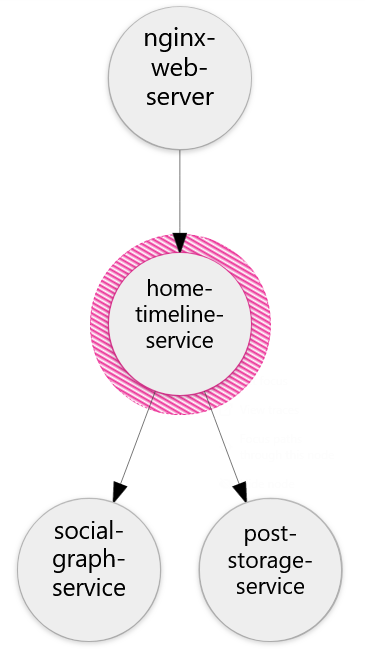
\includegraphics[width=1.0\linewidth]{Figures/Home-Timeline-GET-Trace.png}
    \end{minipage}\hfill
    \begin{minipage}{0.75\linewidth}
        %\caption{Compose Post API trace}
        %\label{fig:compose-post-trace}
        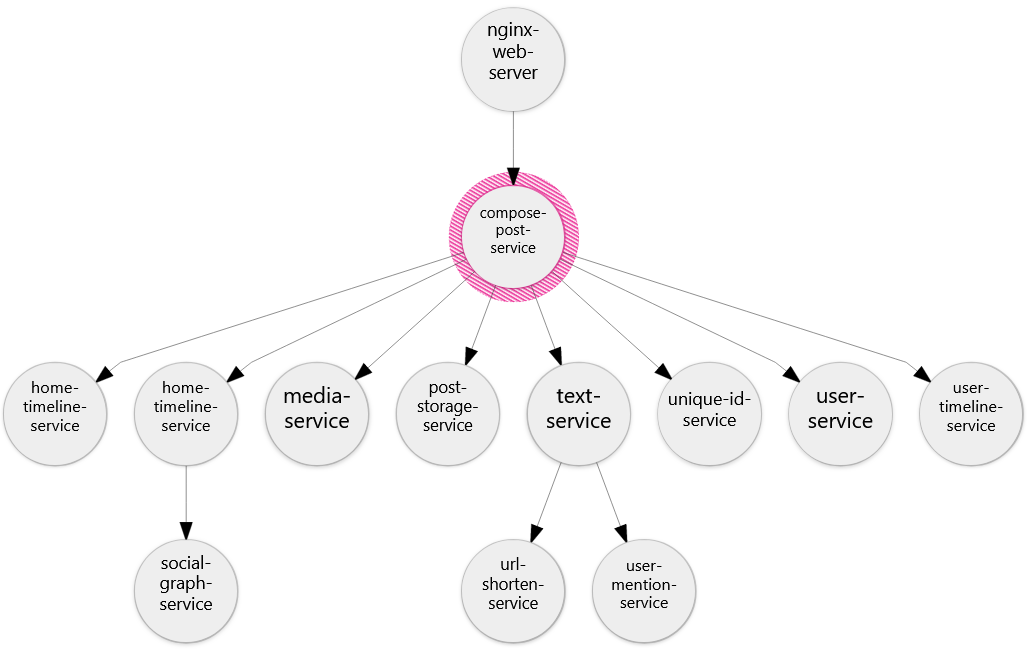
\includegraphics[width=1.0\linewidth]{Figures/Compose-Post-POST-Trace.png}
    \end{minipage}
\end{figure}

\begin{lstlisting}[
  caption={Update resources for bottlenecked deployments},
  captionpos=t,
  label={lst:deploy-resource-update},
  language=bash
]
$ helm upgrade social-media \
/DeathStarBench/socialNetwork/helm-chart/Chart.yaml -n default \
--set-string compose-post-service.container.resources="requests: 
      cpu: "30m"
    limits:
      cpu: "30m"" \
--set-string home-timeline-service.container.resources="requests: 
      cpu: "15m"
    limits:
      cpu: "15m""
\end{lstlisting}

\section{Experiment Setup}
\label{sec:ch5-exp-setup}

Two independent experiments were conducted to verify the performance of the hybrid autoscaler. The social media application was first tested using the GET API to autoscale the home-timeline-service deployment. Then, a more demanding as well as challenging workload was applied to the POST API for autoscaling the compose-post-service deployment. For both these experiments, the workload generation algorithm was used to create realistic daily workloads and tested over the period of one week. Both experiments would configure a flexible SLA latency agreement to be maintained. For the first experiment, the SLA constraint was set to a 150 milliseconds latency, and for the second experiment, it was 1000 milliseconds. The flexible SLA constraint was the primary focus of the experiment, however a moderate and strict SLA constraint was also chosen and tested. The SLA values are shown in table \ref{tab:experiment-sla-values}.\par

%TC:ignore
\begin{table}
    \caption{Experimental SLA constraints}\label{tab:experiment-sla-values}
    \centering
    \begin{tabular}{|l|l|l|}
        \hline
        SLA Type & GET API constraint (ms) & POST API constraint (ms)\\
        \hline
        Flexible    & 150   & 1000\\
        Moderate    & 125   & 900\\
        Strict      & 100   & 800\\
        \hline
    \end{tabular}
\end{table}
%TC:endignore

For the proposed hybrid algorithm to achieve these autoscaling goals within the SLA constraints, the autoscaling subsystems were configured as follows. The reactive autoscaler would check if the CPU utilization of the deployment was exceeding the auto-scaling threshold. This threshold would vary for each of the experiments as required. If so, it would scale up based on the cooldowns and tolerations set. The proactive autoscaler on the other hand would check if the forecasted CPU utilization in the next 20 minutes was going to breach the auto-scaling threshold, and if so, would autoscale with the same configured parameters as the reactive one. The daemon would store the total CPU utilization of the deployment as a time-series for a maximum of seven days, and constantly check for SLA violations to tweak the hyper-parameters of the forecaster as discussed above in section \ref{subsec:ch4-auto-daemon-subsection}. To measure the effectiveness of the hybrid autoscaler, three baseline algorithms were chosen for comparison. All three would autoscale at the same CPU auto-scaling threshold to maintain consistency. Furthermore, these algorithms would be implementations based on the ones discussed in section \ref{sec:ch2-lit-review}.\par

The first was the default Kubernetes horizontal pod autoscaler. No modifications to the configuration were made, thus the scale up cooldown was 0 seconds, while the scale down was 300 seconds. Additionally, the autoscaler had no knowledge of the workload distribution or SLA violations on the edge nodes.\par

The second baseline was an implementation of the reactive traffic aware horizontal pod autoscaler created by Phan et al. \cite{phan2022traffic}. This autoscaler scheduler would compute the ratio of workloads being exerted on the different edge nodes with the deployment pods. Once it did so, it would scale these resources in a commensurate proportion.\par

Finally, the last baseline implementation was the Proactive Pod Autoscaler (PPA) devised by Ju et al. \cite{ju2021proactive}. This algorithm was an open-ended implementation which enabled the user to plugin a deep learning model of their choice. The PPA architecture consisted of three sub-sections, the formulator, evaluator, and updater. An LSTM model was injected into the autoscaler as the model file. This LSTM implementation was similar to the one used in the hybrid autoscaler, however it differed in two key elements. First, the LSTM did not expect pre-processed data without noise, and thus dealt with more complex time-series data. Secondly, due to this additional computation, the LSTM contained a deeper architecture layer with more neural network units. This was required as the algorithm had to correctly predict the complete future workload since there was no reactive autoscaler to fall back on. Over a fixed interval, the algorithm continuously looped through the time-series data and saved the forecast result to a metrics file. The evaluator took these outputs from the metrics file, along with the LSTM from the model file to predict the number of pods to assign in advance, and requested the Kubernetes scheduler for scaling through the API Service. A second loop, known as the update loop, then updated the LSTM model using the latest forecast, and cleared the metrics file. The hyper-parameters were carefully tuned to ensure that the model did not under-perform too significantly. Finally, the PPA architecture did not take into account SLA compliance, and thus SLA metrics were not provided as a feedback for hyper-parameter tuning.\par


\section{Experiment I - GET API Workload}
\label{sec:ch5-exp1-get-api}

In the first experiment, the IoT workload generation algorithm was configured to create a workload aimed at mimicking GET requests. By doing so, the $home-timeline-service$ deployment becomes the bottleneck receiving all of the requests, and thus can be tested using the proposed hybrid autoscaler, as well as the three baseline algorithms. As shown above, the autoscaling threshold was set to 50\% total CPU utilization, and the SLA latency threshold was set to 150 milliseconds.\par

\begin{figure}[htb]
    \centering
    \caption{Experiment I - Total CPU utilization}
    \label{fig:exp1-workload}
    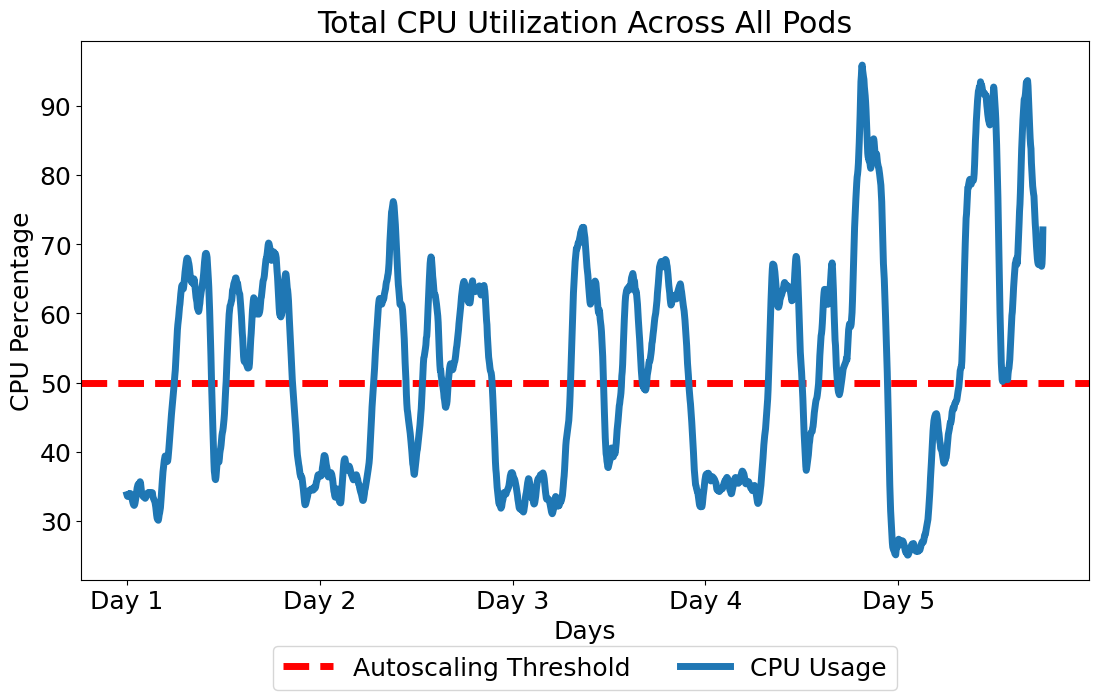
\includegraphics[width=0.6\linewidth]{Figures/GET-Total-CPU.png}
\end{figure}

Figure \ref{fig:exp1-workload} shows the total CPU workload that was generated by algorithm \ref{alg:work-gen} on the $home-timeline-service$ deployment. The data was generated for a total of five days. Each day approximately $510000$ requests were sent to the edge deployment. The daily peak remains at approximately the same percentage, but then increases significantly in the last two days. This can be a depiction of how social network requests may look on the weekends. The total CPU utilization never exceeded 95\% of the total allocated resources shown in listing \ref{lst:deploy-resource-update}. This is expected of a GET request, as while the deployment has to open a connection to the sub-deployments to receive the response, a GET request is typically a database SELECT statement, which takes a comparatively less amount of time as opposed to other operations. This means that the deployment can quickly receive the response from its child components, send the response up to the requester, and then close the connection. Once the connection is closed, all the resources associated with it are freed. Because this operation is so quick, multiple concurrent connections are typically not open, and thus the CPU utilization is not significant.\par

\subsection {Default Kubernetes Autoscaler Baseline}
\label{subsec:ch5-exp1-default-algo}

\begin{figure}[htb]
    \centering
    \caption{Experiment I - Kubernetes Default Autoscaler Latency}
    \label{fig:exp1-default-k8s}
    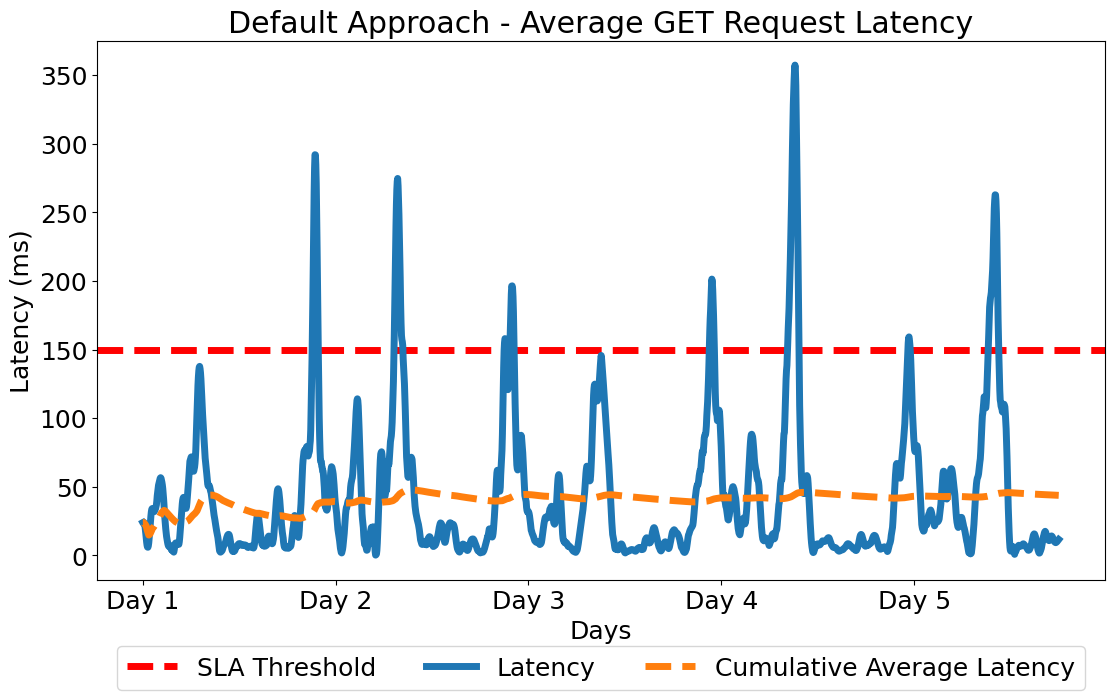
\includegraphics[width=0.6\linewidth]{Figures/Home-Timeline-Default-Latency.png}
\end{figure}

Even with such a workload, a near 100\% CPU utilization on a solitary deployment pod would lead to significant delays. This can be seen when using the default Kubernetes Horizontal Pod Autoscaler, as depicted in figure \ref{fig:exp1-default-k8s}. The autoscaler is merely a primitive reactive implementation with no knowledge of which edge nodes are experiencing heavy traffic, and which ones are not. Thus, it blindly assigns pods to the nodes in a round-robin manner. Additionally, the autoscaler requires a lot of time to register the new pods to the Kubernetes control plane, thus falling victim to the cold start problem. This results in significant latency spikes before the resources are adjusted. In the figure, it can be seen that the latency exceeds 300 milliseconds at some points, which would render the edge deployment unusable. Additionally, by the end of the fifth day of testing, the average latency of the social-network was nearly 50 milliseconds. Through this experiment, it can be concluded that the default Kubernetes autoscaler is completely unsuitable for edge auto-scaling use-cases which are SLA sensitive.\par

\subsection {Reactive THPA Autoscaler Baseline}
\label{subsec:ch5-exp1-reactive-algo}

\begin{figure}[htb]
    \centering
    \caption{Experiment I - THPA Reactive Autoscaler Latency}
    \label{fig:exp1-reactive-k8s}
    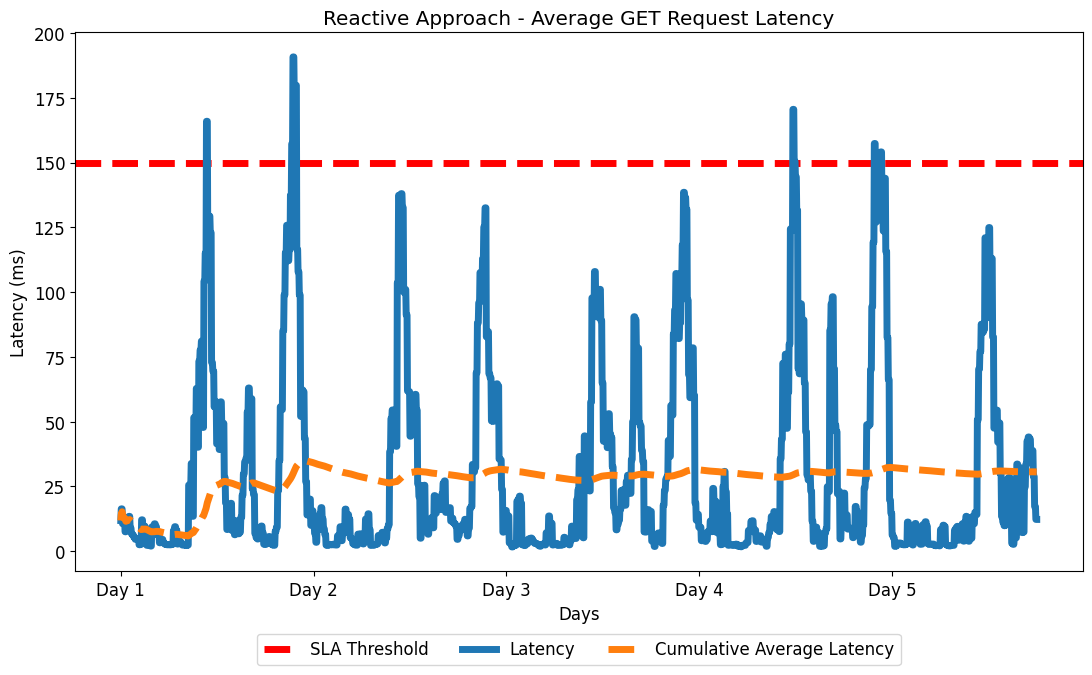
\includegraphics[width=0.6\linewidth]{Figures/Home-Timeline-Reactive-Latency.png}
\end{figure}

The second autoscaling baseline solution to be tested was an in-house implementation of the reactive traffic aware horizontal pod autoscaler solution by Phan et al. \cite{phan2022traffic}. Unlike the default Kubernetes autoscaler, THPA keeps track of which edge node was receiving significant number of requests and assigns pods to the nodes accordingly. This strategy results in a significantly improved latency graph, as can be seen in Figure \ref{fig:exp1-reactive-k8s}. While the algorithm still suffers from the cold start problem, the more intelligent assignment of resources results in less availability issues, ensuring that the latency spikes which are seen are not as drastic as the ones in the default implementation. However, due to the cold start problem, the SLA threshold of 150ms is still regularly breached, resulting in several violations and loss of availability. However these breaches never exceed the 200ms mark, and thus complete loss of system availability is never seen. Furthermore, the average latency over the experimental time frame was lower than what was seen in the default implementation, hovering at around 25-30 milliseconds. Therefore, the reactive approach, while a valid solution for most edge solutions, is not adequate for an SLA-constrained architecture, and further modifications are required.\par

\subsection {Proactive PPA Autoscaler Baseline}
\label{subsec:ch5-exp1-proactive-algo}

The final baseline algorithm to be deployed for auto-scaling $home-timeline-service$ was an implementation of the proactive pod autoscaler (PPA) based on Ju et al. \cite{ju2021proactive}. Unlike the previous two baseline algorithms, this one attempts to predict the workload before it is requested, thus eliminating the cold start issue. In ideal conditions, this would result in the SLA threshold not being violated, and it being a viable solution for edge paradigms. However, experimental results showed otherwise.\par

\begin{figure}[htb]
    \centering
    \caption{Experiment I - PPA Proactive Autoscaler Latency}
    \label{fig:exp1-proactive-k8s}
    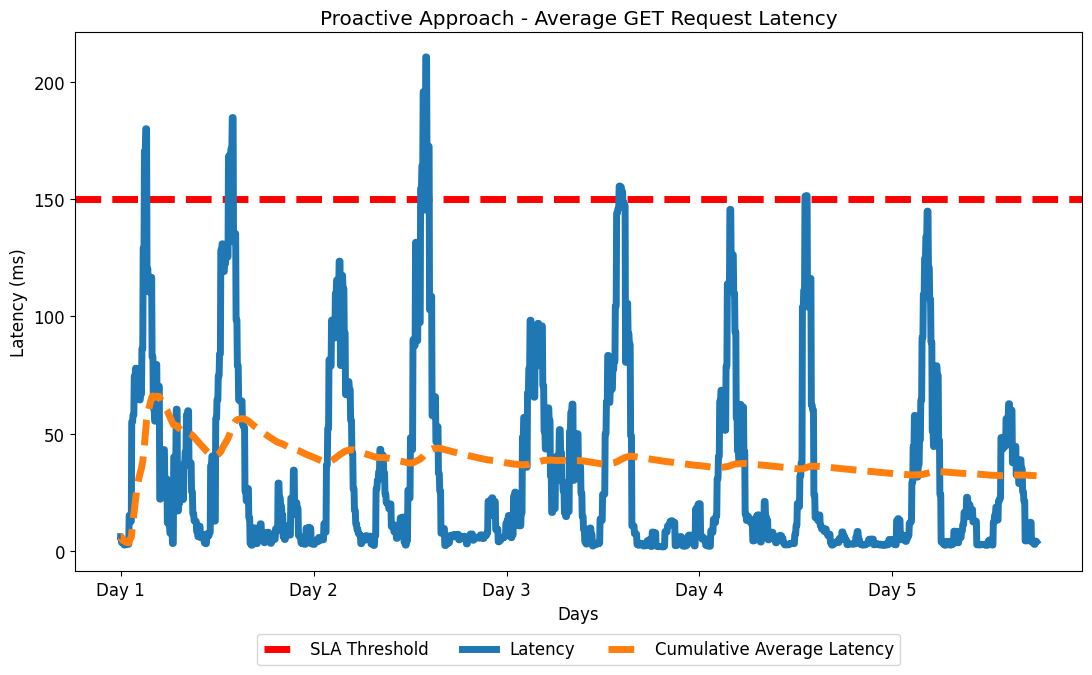
\includegraphics[width=0.6\linewidth]{Figures/Home-Timeline-Proactive-Latency.png}
\end{figure}

Because the autoscaler is purely proactive, it must be a deep LSTM model with several layers and large training epochs. This deep model takes more than 20 minutes to properly train and validate for it to predict 24 hours of data, similar to what our proposed hybrid solution predicts. This is due to the edge architectures lack of resources and storage compared to the cloud layer. Figure \ref{fig:exp1-proactive-k8s} shows this in action. Initially it is observed that the latency continually spikes, causing a large amount of SLA violations, more than what the reactive autoscaler caused. However, after a few days of training, the rolling update structure of the LSTM weights took over, reducing the training time by taking advantage of the early stopping callback in the LSTM model, and managing to stabilize the latency. However, this affect does not always manage to stem the latency overflow, as is shown when the same algorithm was tested using the POST API in section \ref{subsec:ch5-exp2-proactive-algo}.

While the SLA violations were not as severe as the ones seen in the Default autoscaler baseline, they were comparatively greater than the reactive approach, with the latency exceeding 200 milliseconds for several minutes during the day, causing a loss of availability. The average latency was almost as large as what was seen in the default autoscaler baseline, approaching 50 milliseconds due to the issues inherent in attempting to forecast the entire time-series data curve.  Due to these issues, the algorithm itself was demonstrated as unsuitable for SLA-constrained paradigms.\par

\subsection {Proposed Hybrid Autoscaler}
\label{subsec:ch5-exp1-hybrid-algo}

\begin{figure}[htb]
    \centering
    \caption{Experiment I - Hybrid Autoscaler Latency}
    \label{fig:exp1-hybrid-k8s}
    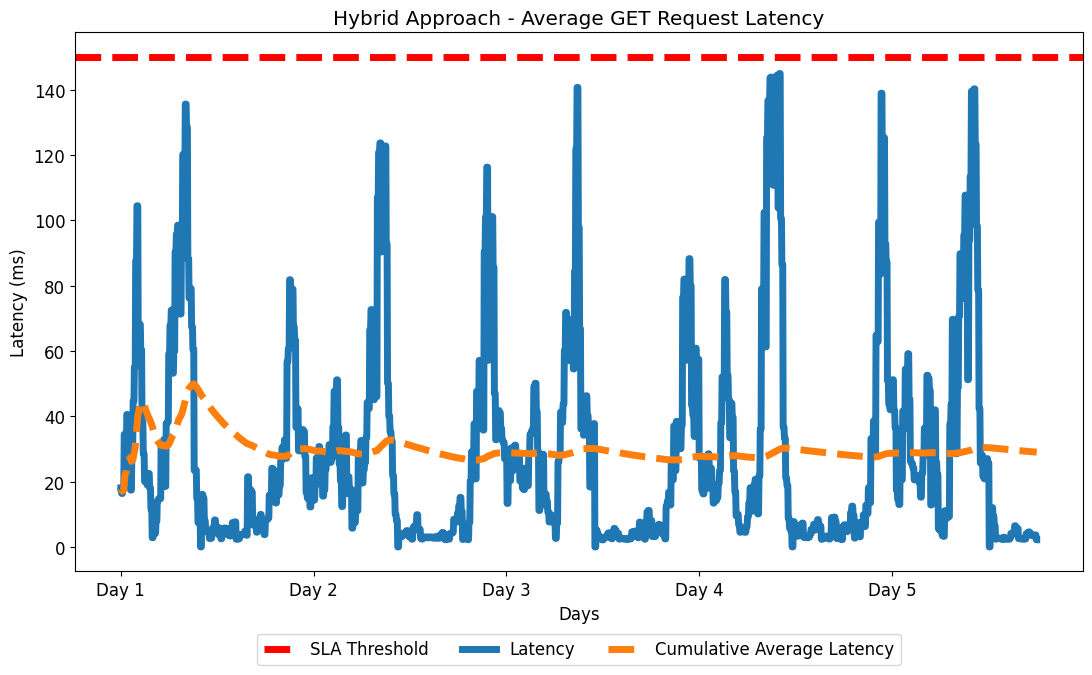
\includegraphics[width=0.6\linewidth]{Figures/Home-Timeline-Hybrid-Latency.png}
\end{figure}

Finally, with the baselines being established in a default, reactive, and proactive approach, the hybrid algorithm was tested on the five days of generated workload. This approach demonstrated how it could mitigate the issues seen in both reactive and proactive auto-scaling approaches. The autoscaler was extremely lightweight, and easy to configure, since there was no hyper-parameter tuning required. Building on top of this light weight, the proactive forecaster was able to forecast the beginning of the workload spike accurately, thus leading to it eliminating the issue of cold start. The forecaster could not accurately predict the middle and end of the daily workloads, however this was not an issue, since the reactive algorithm was capable of taking over the auto-scaling process, and maintaining the necessary resources to avoid SLA violations. Figure \ref{fig:exp1-hybrid-k8s} shows the complete latency graph for the hybrid experiment.\par

From the graph, it is clear that for the GET request experiment, no SLA violations were present for the duration of the five day workload. Thus in this case, the autoscaler daemon did not require to kick in and modify the hyper-parameters of the forecaster. The average latency experienced by the social network is also comparatively low, achieving results similar to the THPA reactive implementation with the value hovering at around 30 milliseconds. This performance is a significant improvement over the baseline algorithms, and demonstrated the efficacy of such a model in an edge architecture deployment.\par


\subsection {CPU Workload Distribution Per Autoscaler}
\label{subsec:ch5-exp1-workload-dist}

The distribution of CPU workload across the deployment pods was another important metric to factor in to the analysis. With an autoscaler threshold being set at $\mathcal{A}$, ideally the distributed workload should hover at $\frac{\mathcal{A}}{2}$. When this workload distribution value $workload \rightarrow \mathcal{A}$ such that the total CPU workload being exerted on each pod is not putting a burden on the social network, driving up latency. On the other hand, when $workload \rightarrow \mathcal{0}$, the returns when it comes to latency reduction are extremely low, while the number of resource pods being assigned to the deployment undergoing auto-scaling are increasing significantly. This in turn increases the cost of running the underlying edge architecture, making this autoscaler an unprofitable alternative.\par

\begin{figure}[htb]
    \centering
    \caption{Experiment I - Autoscaler CPU Workload Distribution Comparison}
    \label{fig:exp1-cpu-avg-dist}
    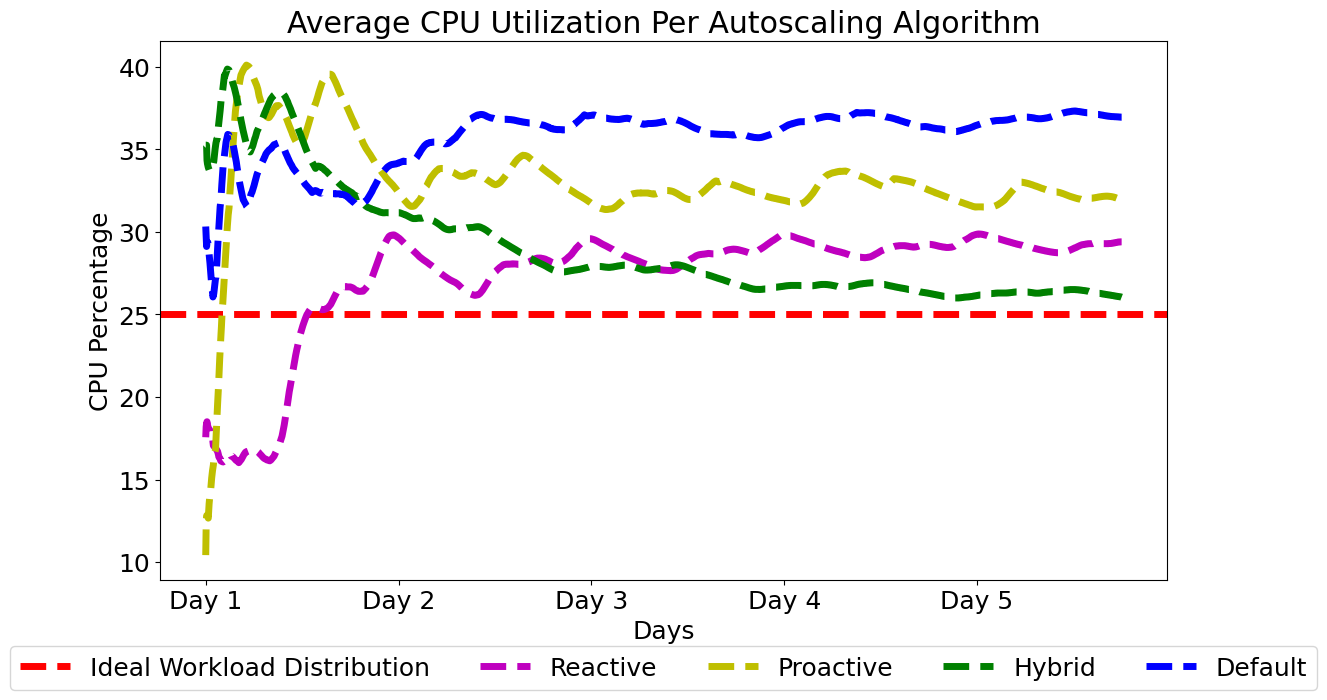
\includegraphics[width=0.6\linewidth]{Figures/Home-Timeline-CPU-Usage.png}
\end{figure}

Figure \ref{fig:exp1-cpu-avg-dist} shows the average CPU utilization of all the deployment pods for the three baseline algorithms, and the proposed hybrid solution. As expected, the default Kubernetes horizontal pod autoscaler performs the worst, with the average utilization hovering around 35\%. The proactive forecaster has a utilization of approximately 33\%, with it being held back by the forecaster complexity and resource intensive training. The reactive approach was the most lightweight autoscaler, and thus performed well with the CPU utilization of around 30\%. Finally, the hybrid autoscaler performed the best of the four compared algorithms, with the utilization of approximately 26\%. This demonstrates that, while the hybrid approach is able to mitigate or eliminate SLA violations, it does so in a manner which is both using a lightweight deployment, and with an algorithm which does not deploy resources in a wasteful manner.\par

\subsection{SLA Violations Analysis}
\label{subsec:ch5-exp1-sla-violations}

As demonstrated above, the hybrid autoscaler performed significantly better than the baseline approaches. However, this was only compared using the flexible SLA thresholds. As a reminder, this was the most lenient threshold possible. For a more thorough demonstration, the algorithms needed to be tested on other thresholds.\par

To achieve this, all four algorithms were tested again on the moderate and strict SLA violation thresholds for the GET API, as displayed in table \ref{tab:experiment-sla-values}. The IoT workload generation algorithm was once again used to generate this, however this time the workload was run for two days. This was done to get the SLA violation percentage for approximately 1.02 million GET requests.\par

\begin{figure}[htb]
    \centering
    \caption{SLA Violation Percentage For GET API Thresholds}
    \label{fig:exp1-sla-violation-bar}
    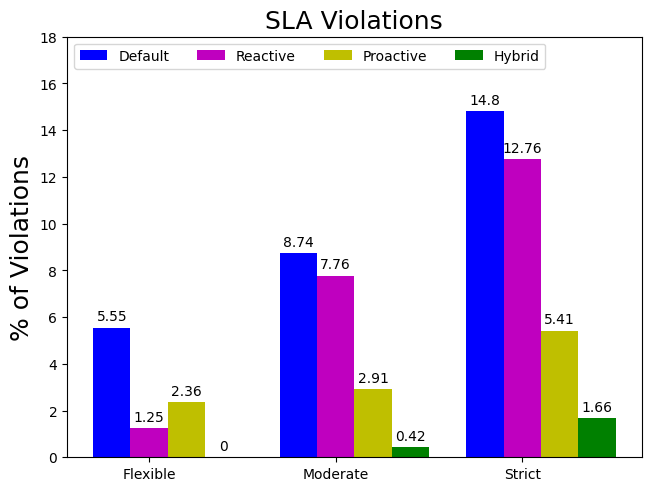
\includegraphics[width=0.6\linewidth]{Figures/Home-Timeline-SLA-Violations.png}
\end{figure}

Figure \ref{fig:exp1-sla-violation-bar} shows the SLA violations for the three different categories. The flexible percentages are taken from the data taken from the five day experiment using the 150 millisecond threshold. The default Kubernetes autoscaler performed the worst, with 5.55\% of all requests being above the SLA threshold. The proactive PPA algorithm came next with a violation rate of 2.36\%, with the amount of violations being increased due to the complexity of the training model. The reactive THPA algorithm performed well, the low resource deployment, combined with the low overhead of GET requests ensured that it only violated the SLA thresholds of 1.25\% of requests. Finally, as seen above, the hybrid autoscaler performed the best of the four implementations, being able to serve all the requests with a 0\% SLA violation rate. This would qualify the hybrid architecture for a ``highly available'' SLA deployment.\par

While the flexible SLA threshold showed impressive results for three out of the four algorithms, the moderate threshold of 125 milliseconds was a more difficult constraint to maintain. The importance of the cold start problem when it comes to SLA latency was exposed in this threshold, as the default Kubernetes implementation and the reactive THPA autoscaler showed extremely similar results, violating 8.74\% and 7.76\% of requests respectively. On the contrary, the proactive PPA approach was able to demonstrate how even mitigating the cold start problem while not being able to eliminate it completely can still have benefits, with the algorithm violating just 2.91\% of requests. Finally, the hybrid autoscaler still achieved the best results. There were violations at the beginning of the experiment, resulting in 0.42\% of requests being above the SLA threshold. However, this was quickly counteracted by the autoscaler daemon, which modified the hyper-parameters to stabilize the latency. Once this was achieved, the hyper-parameters were dropped back down to the default values, and the autoscaling continued as normal.\par

Finally, the strict SLA threshold of 100 milliseconds was tested, which proved extremely difficult to comply with. Once again, the default and reactive autoscalers performed similarly poorly, with 14.8\% and 12.76\% of requests not meeting the SLA threshold respectively. The proactive algorithm distinguished itself from the reactive ones, clearly showing the importance of the cold start problem, by only violating 5.41\% of the requests. However, in this scenario as well, the hybrid algorithm performed significantly better with only 1.66\% of violations. Even though the algorithm would occasionally violate the threshold, the combined approach, along with the daemon's heuristic feedback was able to control the violation rate far better than the three baseline approaches.\par

In conclusion, the hybrid approach proved to be the best autoscaler when it came to an edge deployment with minimal resources available. Furthermore, the algorithm was adaptable, able to display considerably improved performance in comparison with other reactive and proactive approaches using different SLA thresholds. It was able to achieve this with minimal parameter configurations required by the user. The total number of requests, along with the number of violations is provided in the table \ref{tab:exp1-sla-violation-count}.

%TC:ignore
\begin{table}
    \caption{Get Request SLA Violation Counts For The Autoscalers}\label{tab:exp1-sla-violation-count}
    \centering
    \begin{tabular}{|l|l|l|l|l|}
        \hline
        Request Count(M) & Default & Reactive(M) & Proactive(M) & Hybrid(M)\\
        \hline
        Flexible - 25.5  & 1.415 & 0.319 & 0.602 & 0\\
        Moderate - 10.2 & 0.89 & 0.79 & 0.30 & 0.04\\
        Strict - 10.2 & 1.51 & 1.30 & 0.55 & 0.17\\
        \hline
    \end{tabular}
\end{table}
%TC:endignore


\section{Experiment II - POST API Workload}
\label{sec:ch5-exp2-post-api}

The first experiment focused on auto-scaling a resource deployment which was relatively easier to maintain SLA-constraints on. As seen in section \ref{sec:ch5-exp1-get-api}, the GET API does not maintain as many connections simultaneously, meaning a well designed algorithm can achieve 0\% violations on a flexible SLA threshold. \par

For the second experiment, the focus was on a more difficult auto-scaling task. The IoT workload generation algorithm \ref{alg:work-gen} was reconfigured to simulate a realistic workload for social network users writing user timeline posts, which at a low level, involve sending POST requests to the edge deployment.
Doing so meant that the $compose-post-service$ would be sending all these POST requests to its sub-components for writing media or text. The workflow for a POST request goes as follows. The user sends a POST request with the body containing the data to be written. This is sent to the $compose-post-timeline$ deployment which opens an ephemeral connection with the user. Simultaneously while doing so, the deployment sends the contents of the POST body to one of its sub-components. These components house the database for user posts, and the operation is performed using an INSERT statement. The sub-component then sends its response back to the $compose-post-service$ informing it whether or not this operation succeeded or failed. The deployment sends this information back up to the user and closes the connection.\par

\begin{figure}[htb]
    \centering
    \caption{Experiment II - Total CPU utilization}
    \label{fig:exp2-workload}
    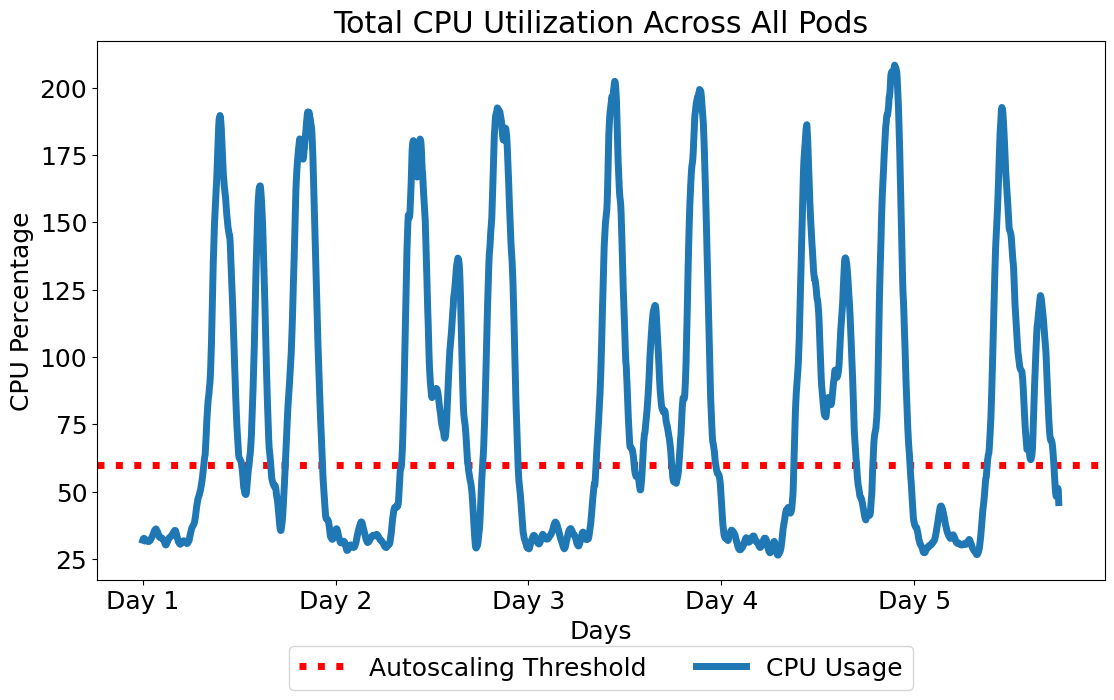
\includegraphics[width=0.6\linewidth]{Figures/POST-Total-CPU.png}
\end{figure}

While the SELECT statement used underneath the GET request was a fairly quick operation, the INSERT statement may take significantly longer, due to the idempotent nature of the database. The social network will ensure that user posts are in the correct order, and perform other background checks before committing the data. Due to this, the open connection on the $compose-post-service$ can remain for a significantly longer amount of time, resulting in far more resources being used. Figure \ref{fig:exp2-workload} shows this in action. The algorithm was generated for a total of 5 days, similar to the first experiment. Even though the workload generation algorithm was sending the same amount of POST requests as it did GET requests, approximately $510000$ requests per day, the total CPU workload in the second experiment peaks at approximately 175\%, and some times even reaches 200\% of the total CPU resources assigned to a unitary deployment pod. This varies per day in a realistic manner similar to what could commonly be seen in social networks.\par

To resolve this CPU bottleneck, the auto-scaling threshold was set to 60\% of the CPU workload. In addition, the SLA latency threshold was set to 1000 milliseconds. Using these configurations, the three baseline algorithms along with the proposed hybrid autoscaler was tested.\par

\subsection {Default Kubernetes Autoscaler Baseline}
\label{subsec:ch5-exp2-default-algo}

\begin{figure}[htb]
    \centering
    \caption{Experiment II - Kubernetes Default Autoscaler Latency}
    \label{fig:exp2-default-k8s}
    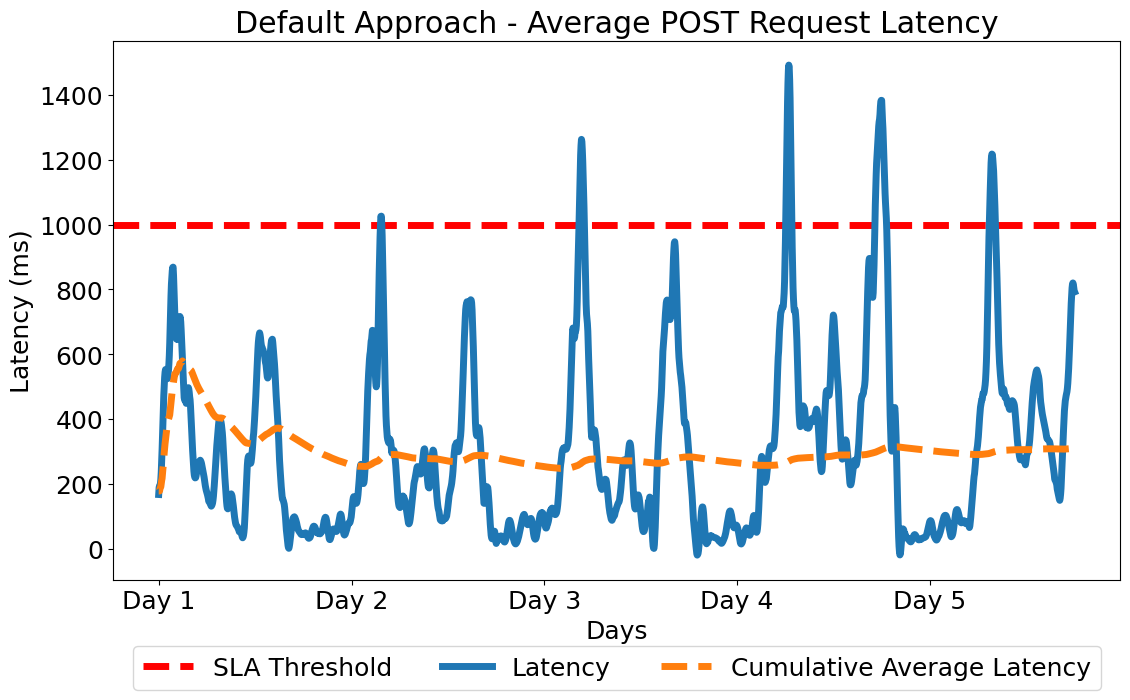
\includegraphics[width=0.6\linewidth]{Figures/Compose-Post-Default-Latency.png}
\end{figure}

To establish a baseline, the first algorithm to be used to scale the deployment was the default Kubernetes Horizontal Pod Autoscaler. This was the same primitive reactive implementation which was seen in section \ref{subsec:ch5-exp1-default-algo}. Similar to that experiment, the shortcomings of this approach was exposed even more so by the increased demands of the POST workload. Figure \ref{fig:exp2-default-k8s} shows the latency metrics of the autoscaler. During the daily workload spikes, the autoscaler would regularly breach the 1000 millisecond threshold, with values peaking at almost 1450 milliseconds. This is more than 45\% above the allowed threshold, which would cause system unavailability.\par

Upon further investigation, it was discovered that the high latency was caused due to two issues. One is the cold start problem, which adds a constant latency to the non-proactive algorithms which cannot be solved by any reactive ones. The second one is the avalanche affect which is caused by resources not being available in a timely manner, and is related to the cold start. Before the Kubernetes control plane can register all resources, the $compose-post-service$ deployment may have a CPU utilization of 100\%. When this happens, the deployment already has all available resources being utilized to open connections, this causes additional connection requests to be dropped. The user does not see this happen, and instead waits the default 60 seconds before displaying a ``time-out'' message. This 60 seconds is considered when measuring the latency, and is what drives up the latency so much. Furthermore, the Kubernetes default autoscaler has no information on which edge nodes are receiving the most number of requests. It only sees CPU utilization metrics as a totality. As a result of this, it schedules new resources in a round-robin manner, meaning that some deployment pods receive a lot of requests, while others may receive none. This uneven distribution of requests to the resources also drives up latency.\par

Based on these experimental results which showed that connections were being dropped, it meant that the social network was becoming unavailable at certain points in time during the day. This happening during peak hours was especially critical, and violated SLA constraints. Due to this, the default Kubernetes autoscaler could not be considered viable for auto-scaling an edge deployment.

\subsection {Reactive THPA Autoscaler Baseline}
\label{subsec:ch5-exp2-reactive-algo}

The second baseline algorithm to be tested was the traffic aware horizontal pod autoscaler designed by Phan et al. \cite{phan2022traffic}. This reactive algorithm was expected to face the cold start issue seen in the default Kubernetes autoscaler, but mitigate some of the dropped requests which were causing the latency to exponentially increase.\par

\begin{figure}[htb]
    \centering
    \caption{Experiment II - THPA Reactive Autoscaler Latency}
    \label{fig:exp2-reactive-k8s}
    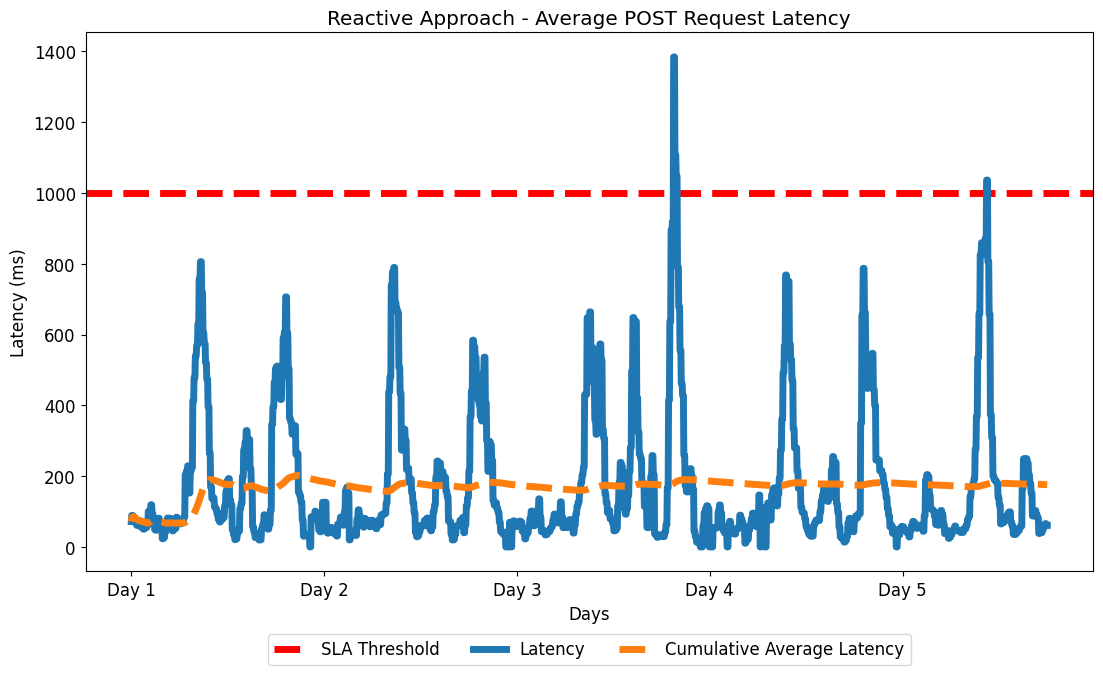
\includegraphics[width=0.6\linewidth]{Figures/Compose-Post-Reactive-Latency.png}
\end{figure}

Figure \ref{fig:exp2-reactive-k8s} shows how the THPA algorithm performs on the workload. As was expected, the request-aware architecture of this autoscaler allowed it to eliminate the issues with dropped requests seen above. This was due to the autoscaler assigning resource pods to the edge nodes which were experiencing high number of POST requests. This ensured that on an average, the latency values were kept lower. Furthermore, the avalanche affect seen above was somewhat mitigated due to the more intelligent resource deployment model.\par

However, the cold start problem was not eliminated, which caused spikes in the latency when the autoscaler could not handle assigning resources in time. While this was less common in this implementation than in the default one, it nevertheless resulted in latency spiking above the SLA threshold for lengthy amounts of time on multiple occasions. On one occasion, the latency nearly hit 1400 milliseconds for several minutes before coming back down when the resource registration was completed.\par

These issues were not as severe as the ones seen in the default autoscaler however, and would not cause complete system unavailability. However, SLA was still being violated regularly, and thus while the autoscaler can be considered as a suitable algorithm for native cloud deployments, it was deemed unsuitable for edge deployments with SLA constraints.\par

\subsection {Proactive PPA Autoscaler Baseline}
\label{subsec:ch5-exp2-proactive-algo}

The third and final baseline algorithm to be tested on this workload was the proactive pod autoscaler created by Ju et al. \cite{ju2021proactive}. The autoscaler configurations for both experiments were the same, and involved a complex and deep LSTM model. In ideal conditions, this model was expected to mitigate or even eliminate the cold start problem that was seen in the previous two baseline auto-scaling implementations. While this was the case, the experimental results showed SLA violations still regularly occurred.\par

\begin{figure}[htb]
    \centering
    \caption{Experiment II - PPA Proactive Autoscaler Latency}
    \label{fig:exp2-proactive-k8s}
    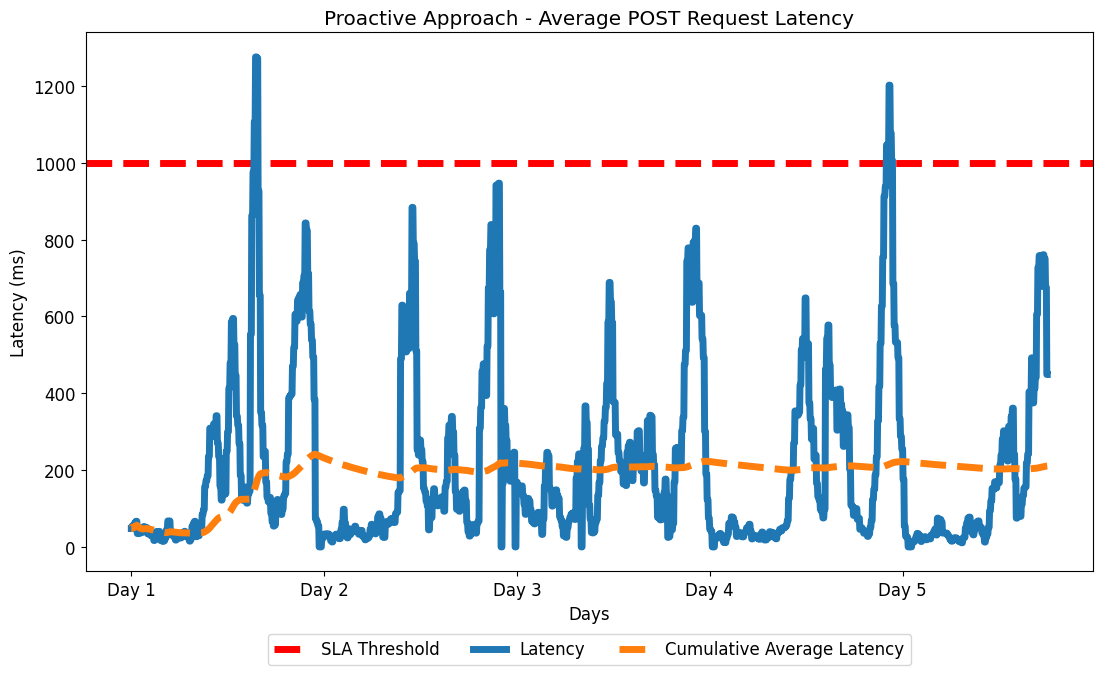
\includegraphics[width=0.6\linewidth]{Figures/Compose-Post-Proactive-Latency.png}
\end{figure}

Figure \ref{fig:exp2-proactive-k8s} shows the full latency graph for the social network. As can be seen from the data, the latency initially spiked to above 1200 milliseconds, before stabilizing below the SLA threshold. However, one more spike occurred on the last day.\par

Further investigations were conducted to attempt to explain why these spikes occurred. It was deduced that the first latency spike occurred due to a shortage of training data. The LSTM used by the PPA architecture is extremely complex. Furthermore, apart from data normalization, no other data pre-processing was done such as passing it through the Savitsky-Golay smoothing algorithm. These issues make it more difficult for the forecaster to correctly predict data curves early on in its development. This issue was resolved as more data was added to the training time-series input, however, after a certain point, a threshold was reached where the data was so large, it took a significantly large amount of time for the autoscaler to forecast the workload. This issue led to the latency spike on the final day leading to SLA violations, lasting for several minutes before the autoscaler corrected itself.\par

From these investigations, it can be seen that the proactive auto-scaling approach worked significantly better than the default Kubernetes autoscaler, but slightly worse than the reactive approach. While the social network POST requests were never dropped which would lead to complete system unavailability, the SLA constraints were nonetheless breached, due to the lack of edge layer resources and large training times for the proactive model. Due to issues such as this, the algorithm could not be considered suitable for edge deployments which were reliant on SLA constraints.\par

\subsection {Proposed Hybrid Autoscaler}
\label{subsec:ch5-exp2-hybrid-algo}

Finally, the hybrid auto-scaling solution proposed in this thesis was deployed to auto-scale the $compose-post-service$ deployment. Once again, the autoscaler was configured the same as in Experiment I, with the only difference being the SLA threshold for heuristic feedback in the autoscaler daemon being reconfigured to 1000 milliseconds. From the above baseline tests, it can clearly be seen that the primary issues faced by the algorithms were the cold start problem, the time taken to predict the complete the forecaster training, and the issue of user requests being dropped due to a lack of resources on nodes with a high CPU usage. Thus, it was hoped that due to the light weight of the algorithm, along with the pre-processing of data and heuristic feedback loop, these issues could be mitigated or even eliminated.\par

\begin{figure}[htb]
    \centering
    \caption{Experiment II - Hybrid Autoscaler Latency}
    \label{fig:exp2-hybrid-k8s}
    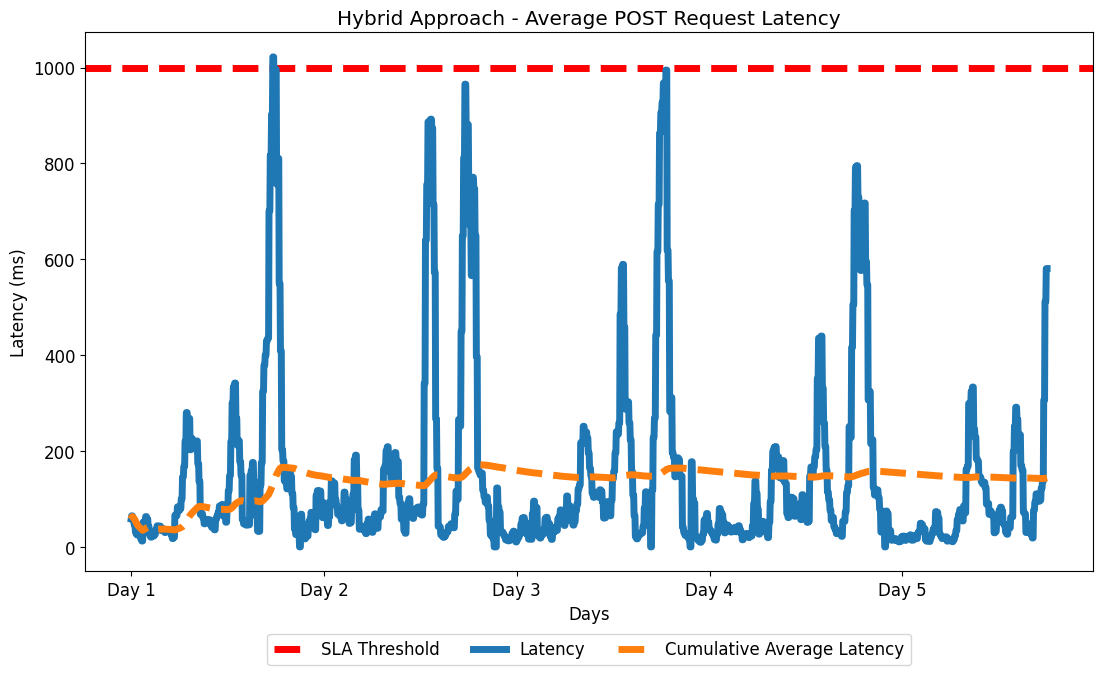
\includegraphics[width=0.6\linewidth]{Figures/Compose-Post-Hybrid-Latency.png}
\end{figure}

Figure \ref{fig:exp2-hybrid-k8s} shows the latency metrics for the five day workload simulation period. From the graph, it can be clearly seen that only one SLA violation took place on the first day. This was a result of the lack of training data causing an erroneous prediction, an issue faced by the proactive baseline algorithm as well. However, what set this algorithm apart from that baseline was that the reactive autoscaler subsystem was capable of taking over from the proactive subsystem and scale the resources accordingly. Due to this, the SLA threshold was only breached slightly, peaking at around 1020 milliseconds.\par
After this SLA violation, the autoscaler daemon reported this back to the forecaster, and deduced that the training process needed to be kick-started through hyper-parameter tuning. This was done in the next training cycle, and as a result, it can be seen that no SLA violations took place on the next day. As a result, the autoscaler daemon reset the hyper-parameters to speed up the training process, and even though the latency approached 990 milliseconds on the third day, no further violations took place for the rest of the simulation.\par

From these tests, it was clear that the hybrid approach had nearly eliminated the cold start problem very early on in the experiment. The initial difficulties in correctly forecasting the workload peaks were quickly resolved by the autoscaler daemon's corrective instructions. All this was done with no user intervention, making the autoscaler extremely autonomous. Furthermore, the algorithm was capable of completing the training within a few minutes, allowing it to finish resource registration quickly. This meant that the CPU utilization of each pod on the nodes never exceeded 100\%, and thus no user POST requests were dropped, allowing for full system availability.\par

Based on these results, it was experimentally demonstrated that the proposed hybrid autoscaler performed far better than the baseline algorithms, only slightly breaching the SLA threshold, while causing no system unavailability. Thus, the efficacy of this hybrid approach for an edge deployment was proven.

\subsection {CPU Workload Distribution Per Autoscaler}
\label{subsec:ch5-exp2-workload-dist}

As demonstrated above, the workload simulation showed the importance of maintaining a low average CPU workload across the deployment pods. If the average CPU utilization is too high, the resource availability would decrease, resulting in connections being dropped, causing the average latency of the social network to drastically increase. On the other hand, if the average CPU utilization is very low, it would mean that an excess of pods had been deployed, most of which were not being used to serve requests. This results in high system deployment costs leading to an unprofitable auto-scaling solution, while not reducing latency by a significant amount.\par

With the auto-scaling threshold of this experiment $\mathcal{A}$ set to 60\%, the ideal distributed workload achieved by the autoscaler should be half of the threshold, as calculated in the first experiment. Thus, the distributed workload for this experiment should be $\frac{60}{2} = 30\%$

\begin{figure}[htb]
    \centering
    \caption{Experiment II - Autoscaler CPU Workload Distribution Comparison}
    \label{fig:exp2-cpu-avg-dist}
    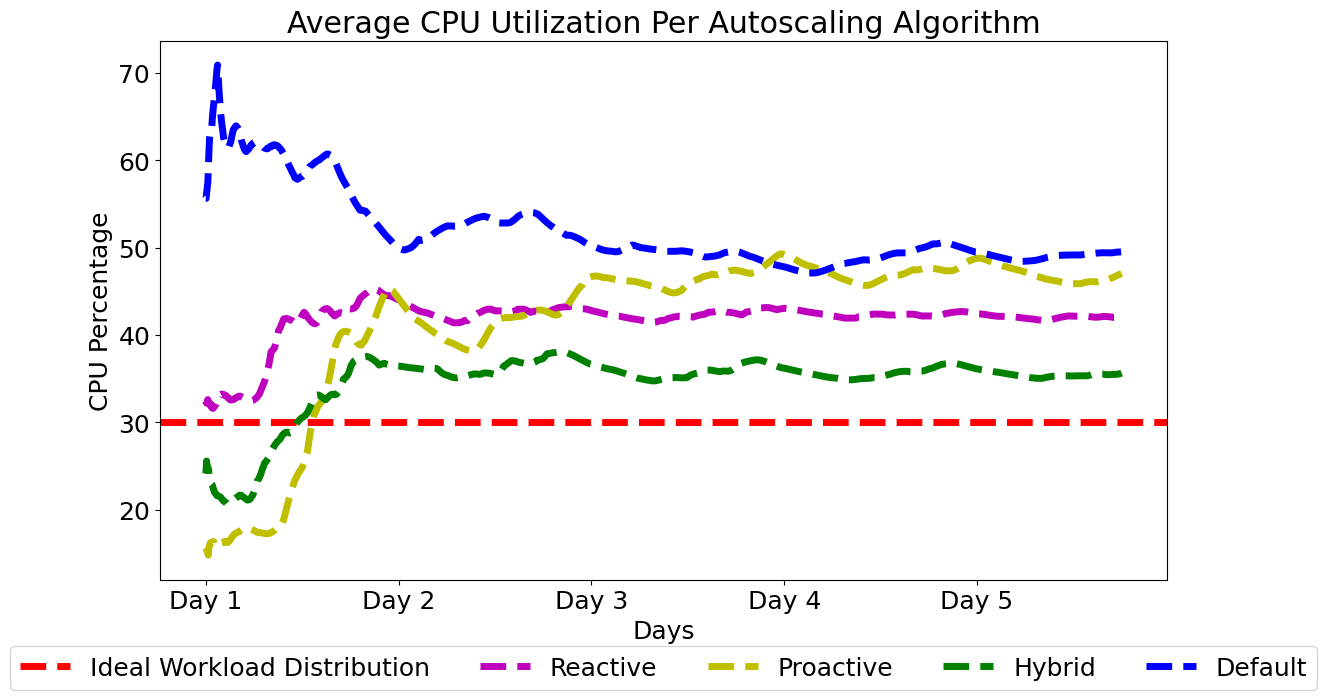
\includegraphics[width=0.6\linewidth]{Figures/Compose-Post-CPU-Usage.png}
\end{figure}

Figure \ref{fig:exp2-cpu-avg-dist} shows the average CPU utilization of the pods being scaled in the deployment by the three baseline algorithms, along with the proposed hybrid solution. As shown above in section \ref{subsec:ch5-exp2-default-algo}, the default Kubernetes autoscaler faced issues with system unavailability, with user requests being dropped. This was caused by high CPU usage on the pods, with this being demonstrated by the graph. The average utilization peaked at around 70\% before stabilizing at around 50\% for all the resource pods. However, it is important to note that these resources were not distributed equitably, and thus while some pods had close to 100\% utilization, others had near 0\%.\par

The baseline proactive PPA algorithm performed third best. While its CPU utilization stabilized fairly quickly to a value of approximately 45\%, this was still far higher than the ideal distributed workload. This was most likely caused by the time it took for the algorithm to forecast data due to the complexity of the LSTM model, which resulted in resources lacking for certain periods of time.\par

The reactive THPA algorithm performed second best, with an average CPU utilization of approximately 42\%. This was achieved due to the intelligent placement of pods in the edge nodes through its traffic-aware algorithm. However, the autoscaler was still prone to the cold start problem, and thus there were several occasions where the CPU workload would peak before the appropriate resources could be assigned. Due to this, the average workload was still far higher than the ideal value.\par

Finally, it can be seen from the graph that the hybrid autoscaler performed better than all three of the baseline algorithms. Its proactive subsystem allowed it to nearly eliminate the cold start problem, while its short training times, and reactive subsystem, allowed the efficient placement of resource pods on the deployment. The average CPU workload quickly stabilized to approximately 35\%, which is far lower than the averages we have seen above for the baseline algorithms, and close to the ideal value of 30\%.\par

Through this comparison, it was clearly demonstrated that for multiple use-cases, the hybrid autoscaler managed to scale resources in a manner which both mitigated SLA violations, while doing so in a manner which was both light-weight enough for edge deployments, and inexpensive too.\par

\subsection{SLA Violations Analysis}
\label{subsec:ch5-exp2-sla-violations}

While the hybrid autoscaler was shown to perform significantly better than the baseline approaches, this was only shown using the flexible SLA threshold of 1000 millisecond, which was the most lenient one possible for the POST request use case. For a more robust demonstration, the algorithms needed to be tested on other thresholds as well.\par

To accomplish this, the three baseline algorithms and the proposed hybrid algorithm were tested once more on the moderate and strict SLA thresholds. These thresholds for the POST API were defined in table \ref{table:sla-availability}. The workload generation algorithm was used to generate data for these two use cases for two days each. By doing so, approximately 1.02 million POST requests were generated in total to determine the SLA violation percentage.\par

\begin{figure}[htb]
    \centering
    \caption{SLA Violation Percentage For POST API Thresholds}
    \label{fig:exp2-sla-violation-bar}
    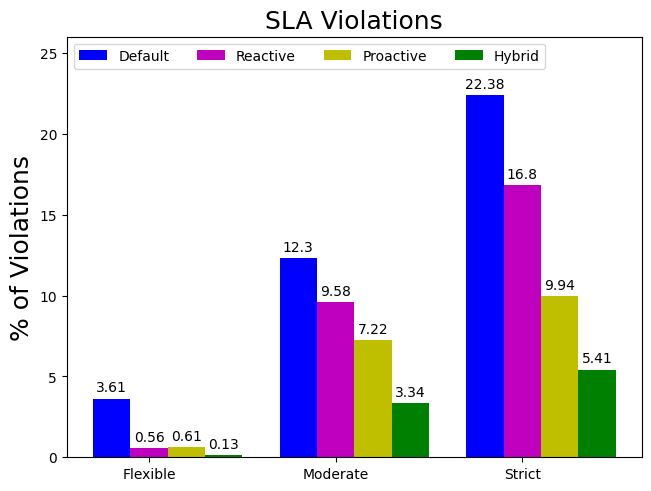
\includegraphics[width=0.6\linewidth]{Figures/Compose-Post-SLA-Violations.png}
\end{figure}

Figure \ref{fig:exp2-sla-violation-bar} depicts the SLA violations for all four algorithms for the three SLA categories. Once again, the flexible percentages were derived from the data taken during the five day experiment using the 1000 millisecond threshold, while the moderate (900 millisecond) and strict (800 millisecond) thresholds were derived from the two day workload above.\par

As seen above, for the flexible category, the default Kubernetes autoscaler performed the worst, with 3.61\% of the total requests resulting in an SLA violation. This also includes the requests which resulted in an error due to being dropped by the social network. The reactive and proactive algorithms performed comparatively similar to each other, achieving a 0.56\% and 0.61\% violation rate respectively. The lenient threshold means that the proactive algorithm is unable to display its benefits when it comes to mitigating the cold start problem as compared to the reactive approach. Finally, the hybrid approach achieved a 0.13\% SLA violation rate. This results in approximately 99.9\% availability for the system, indicating that even for a difficult autoscaling task such as for the POST request scenario, the hybrid algorithm is capable of achieving near ``high availability''.\par

The moderate SLA threshold proved far more difficult for all the algorithms to adhere to. Once again, the default Kubernetes autoscaler performed the worst of all four, failing to adhere to the SLA constraint for 12.3\% of the requests. Here, the proactive autoscaler was able to demonstrate the importance of mitigating the issue of cold start. It was able to achieve a 7.22\% of SLA violations, which was far lower than the 9.58\% seen for the reactive autoscaler. However once again, the hybrid solution proved to be the most capable of auto-scaling in this scenario, achieving an SLA violation rate of just 3.34\%.

Finally, the extremely challenging strict threshold was tested. The default Kubernetes autoscaler was unable to cope with such a threshold, violating this threshold for over one-fourth of the requests, with a 22.38\% violation rate. Once again, the proactive algorithm outperformed the reactive one, achieving a 9.94\% violation rate as compared to the 16.8\% of the reactive algorithm. Finally, the hybrid algorithm performed significantly better than all three baselines yet again, with a violation rate of just 5.41\%.\par

This meant that over the two experiments and three SLA thresholds, the hybrid approach served a minimum of 94.5\% of all requests in an SLA-compliant manner in the worst case scenario, while serving 100\% of them in the best case. Through this thorough testing and experimentation, the algorithm displayed its robustness and adaptability while requiring little to no customization by the user to achieve excellent results. The total number of requests, along with the number of request violations is displayed in table \ref{tab:exp2-sla-violation-count}

\suhrid{TODO: Check these table numbers again}
%TC:ignore
\begin{table}
    \caption{POST Request SLA Violation Counts For The Autoscalers}\label{tab:exp2-sla-violation-count}
    \centering
    \begin{tabular}{|l|l|l|l|l|}
        \hline
        Request Count(M) & Default & Reactive(M) & Proactive(M) & Hybrid(M)\\
        \hline
        Flexible - 25.5  & 0.92 & 0.14 & 0.16 & 0.03\\
        Moderate - 10.2 & 0.89 & 0.79 & 0.30 & 0.04\\
        Strict - 10.2 & 1.51 & 1.30 & 0.55 & 0.17\\
        \hline
    \end{tabular}
\end{table}
%TC:endignore